% !TEX root=../thesis.tex

\chapter{Results}
\label{chapter:results}

\section{List learned, to be removed} % (fold)
\label{sec:list_learned_to_be_removed}

\begin{itemize}
	\item Important characteristics
	\begin{itemize}
		\item Stakeholders 
		\begin{itemize}
			\item Defined relevant stakeholders in a hierarchy for more easy 
			aggregation (stakeholder awareness).
			\item Defined requirements of the stakeholders (what information 
			do they need)
			\item Clearly defined responsibility area per level in hierarchy (
			example in data sets)
		\end{itemize}
		\item Data sets
		\begin{itemize}
			\item Information stored accordingly to stakeholders
			\begin{itemize}
				\item In this case as example, stations defined per 
				responsibility area
				\item Other info is connected to stakeholders through
				stations, for clarification of connected to:
				\item Other info is connected to stakeholders through stations, for clarification of connected to
				see following 3 points:
				\item For crossings between trains, compares on equal 
				station at the same time
				\item Density is between given stations
				\item This means stations are stored per area, and other 
				info is fetched according to this.
			\end{itemize}
			\item Generalize data storage
			\begin{itemize}
				\item Easier to remove or add more data to a data set
				\item When having generalized data storage and generalized 
				aggregation, it means it is much easier to add other type of data sets
			\end{itemize}
		\end{itemize}
		\item Aggregation
		\begin{itemize}
			\item Generalize methods for reuse throughout the hierarchy levels and
			through different types of information
			\begin{itemize}
				\item This could mean generating equal return data structure regardless of
				stakeholder hierarchy level and type of data
				\item Results in a much more general information display
				\item Aggregate over data on the step between data storage and presentation
			\end{itemize}
			\item Aggregate through data from different sources
			\item When the data is relative simple (read for instance count per station), a simple aggregation is averaging the data through different stakeholder hierarchy
			level.
			\item Data presentation view based on current selected stakeholder 
			which in turns determines what should be aggregated and returned to be
			presented
		\end{itemize}
		\item Data retrieval optimization
		\begin{itemize}
			\item Minimize data traffic
			\item Efficient queries to minimize execution time
			\item Generality in storage and queries for scalability both  
			in size and data types needed
			\item External vs local storage?
			\item All in one or independent data storage per information 
			type?
		\end{itemize}
		\item Navigation through time and space
		\begin{itemize}
			\item Have a selectable time intersection for limiting data view
			\item "Zoom" the data in space based on the responsibility area/needs of the stakeholders, in this case, fit the visible section of the map to the relevant stations
		\end{itemize}
	\end{itemize}
\end{itemize}

% section list_learned_to_be_removed (end)

% !TEX root=../../thesis.tex

\section{Workshop 2014-04-04} % (fold)
\label{sec:workshop_2014_04_04}
The first workshops agenda was to help define the stakeholders of the system,
their areas of responsibility, and their needs. The workshop was also meant to 
bring clarity to how the system will relate to these users and their needs.
Attending this workshop was Andreas Amdal Seim (SINTEF), Andreas Dypvik 
Landmark (SINTEF), Rimmert van der Kooij (SINTEF), Nils Olsson (NTNU), Per 
Magnus Hegglund (Jernbaneverket), Magnus Bae (NTNU), and Magnus Krane (NTNU).\\

Perspectives that can be used when viewing the system were discussed
first.
\begin{itemize}
	\item Infrastructur: Segment director, etc.
	\item Traffic division / passenger / train companies.
	\item Delay causes: delay demographic.
\end{itemize}

Interests of users when using the system were then discussed based on the
perspectives.
\begin{itemize}
	\item Uptime, punctuality.
	\item Deviation.
	\begin{itemize}
		\item What?
		\item Where?
		\item When?
	\end{itemize}
	\item Delay time.
	\item Variation.
	\item Changes.
\end{itemize}

Causes that might affect the punctuality was also listed: weather, number of
passengers, capacity utilization, animal accidents, cargo volume.
The causes was concluded not to be included in this project, as the causes is
difficult to prove and get data on.\\

The internal project in Jernbaneverket (section
\Ref{sub:subsection_jernbaneverket}) uses a deviation registry for data to
analyze each stretch on a detail level. To calculate the uptime, presented in
\Ref{sec:railway_operations}, also uses the deviation registry for the needed
data. A problem by using the deviation registry for calculating variation or 
changes, the registry have a five minute filter in which the trains are being 
calculated to be on time.

Two problems were agreed upon that needed to be addressed, the back end and 
the  front end of the system. What kind of data is available and what is 
possible to do with this data? A data set can show both positive and negative 
results, based on what the set are compared too. For instance, easter is not 
on the same week each year and the passenger volume increase during the 
holidays. Data sets ended up being addressed in the second workshop (\Ref{sec:workshop_2014_04_24}). 

As the different stakeholders might have need for different presentation of the
data, different levels of stakeholders and what should be shown in each level 
was discussed. A suggestion was made to have the same perspective through the
levels, but to have selectable views based on roles. \\

At the end of the workshop, three conclusions was made. The first conclusion 
was to have a dashboard next to each marker with relevant data to the current 
stakeholder. The second conclusion was to a interactive list of the
stakeholders which adapted the visual presentation to the selected stakeholder,
presented in \Ref{sec:back_stakeholders}.
The last conclusion was to have a second workshop where the content of the
dashboard should be decided. This resulted in \Ref{sec:workshop_2014_04_24}.

% section workshop_2014_04_04 (end)

\section{Workshop 2014-04-24} % (fold)
\label{sec:workshop_2014_04_24}
The second workshops agenda was to determine what statistical data was 
to be implemented in the dashboard, concluded upon in \Ref{sec:workshop_2014_04_04}.
Attending this workshop was Andreas Amdal Seim (SINTEF), Andreas Dypvik 
Landmark (SINTEF), Rimmert van der Kooij (SINTEF), and Magnus Krane (NTNU).\\

The workshop started with a brainstorming for different data to present in
the map. The different data was ranked on implementation practicality from 1 - 
3 where 1 is unpractical and 3 is very practical; and ranked on the 
desirability of the data from 1 - 3 where 1 is undesirable and 3 is very 
desirable. The brainstorming after ranking is presented in \Ref{table:dashboard_functionality_wants_vs_needs}.
\\

\begin{table}[!h]\small
	\begin{tabularx}{\textwidth}{|X|l|l|l|}
		\hline
		Functionality & Practicability & Desirable & Priority\\
		\hline
		Outstanding errors & 1 & 1 & 1\\
		\hline
		Suspensions & 3 & 1 & 3\\
		\hline
		Variation & 1 & 3 & 3\\
		\hline
		Season effects & 3 & 1 & 3\\
		\hline
		Follow delays & 1 & 3 & 3\\
		\hline
		Speed limits & 3 & 1 & 3\\
		\hline
		Cause & 3 & 2 & 6\\
		\hline
	 	Worst stretch/station/train number & 3 & 2 & 6\\
		\hline
		Traffic density & 3 & 3 & 9\\
		\hline
		Speed restrictions & 3 & 3 & 9\\
		\hline
		Delays & 3 & 3 & 9\\
		\hline
		Crossings & 3 & 3 & 9\\
		\hline
	\end{tabularx}
\caption{Dashboard functionality brainstorming ideas}
\label{table:dashboard_functionality_wants_vs_needs}
\end{table}

Based on the ranking, the decision was made to only implement the data was
ranked as a 3 both on practicability and desirability, presented in the list
below.

\begin{itemize}
  \item Delays
  \item Speed restrictions
  \item Crossings
  \item Traffic density
\end{itemize}

The second part of the agenda, was to determine how the selected data was to be
presented. The decision was made to split the presentation in two parts. The
first was to display aggregated data in the dashboards next to the marker based
on the current stakeholder. The second was to display top 5 lists for delays
and speed restrictions.

\subsection{Crossings} % (fold)
\label{sub:crossings}
One of the problems discussed with crossing was should the system take into 
account the difference between actual crossings and planed crossings or not? 
The difference is hard to calculate as one does not know whether one of the 
trains involved in the planned crossing, was canceled or just delayed. The 
decision was made to present the number of crossings occurred at each station, 
and aggregate the number as one navigates in the stakeholder hierarchy.
%TODO planned crossings, ask Landmark.
% subsection crossings (end)

\subsection{Traffic density} % (fold)
\label{sub:traffic_density}
Several options to present traffic density were discussed, the problem was how
to correctly show the number of trains based on the data available. 
Should the system present each train based on the train numbers and 
calculate for the entire line both ways? Should the system display train 
numbers divided by the segment directors? 

In the workshop it was decided to show the number of trains that passes each 
block segment, based on the data available. When navigating in the hierarchy,
the system shall aggregate the number of trains.

% subsection traffic_density (end)

\subsection{Speed restrictions} % (fold)
\label{sub:speed_restrictions}
Speed restrictions was decided to be presented a marker per restriction, and be
shown between the selected time interval. The data for the speed restrictions
was to be presented in a plot which appeared in the marker for each
restriction.

%In the dashboard it was decided to show the top 5 upper and lower bounds. It was also decided to include a little marker on the map to indicate the location of the speed restriction. 

% subsection speed_restrictions (end)

%\subsection{Delays} % (fold)
%\label{sub:delays}
%TODO
%Since delays can cover a large area depending on how you define it, this had to be properly discussed and defined. Should you follow the Norwegian standard \cite{jernbaneverketPunklighetsTall} of only say that a train is delayed at the final destination or use data from the signal post on the stretches  compared to the schedule? Should you take the variation into account? It was decided to display the sum of the seconds the of delays, and sum of trains arriving to early. These sums would then be displayed in the dashboard and be aggregated according to the level.

% subsection delays (end)

% section workshop_2014_04_245 (end)

% section workshops (end)

% !TEX root=../../thesis.tex

\section{Prototype functionality} % (fold)
\label{sec:prototype_functionality}
As part of answering the research question, a prototype was developed. In this
section we will describe the functionality in the prototype.\\

The prototype is a map based system that presents the information according to
the needs of the stakeholders, as presented in \Ref{fig:map_prototype}. A
intractable list was implemented, presented in \Ref{fig:stakeholder_selection_list},
which gives the functionality to navigate through the stakeholders hierarchy.
The system aggregates the data according to the current selected stakeholder,
as presented in \Vref{sub:back_end_aggregation}. The visual presentation will 
be adapted to the the areas of responsibility of the current stakeholder, 
which will focus the presentation of the data in the geographical area of the 
stakeholder.

To let the stakeholder be able to select different types of information
according to their need, a intractable list was implemented (\Ref{fig:implementation_type_selection}).
By letting the user select the information type to present, the system is able
to present the stakeholders need for different information type according to
their requirements. \Ref{fig:crossings_and_speed_restriction_implementation}
shows the presentation of two different types of information.\\

A method to navigate in time were implemented, as the stakeholders have 
different needs for the level of detail in the presentation of data. The time
navigation were implemented as two input boxes, see \Ref{fig:time_selection_implemented}.
The system uses the time interval set by the user to limit the data to be
processed. 

\begin{figure}[!htbp]
	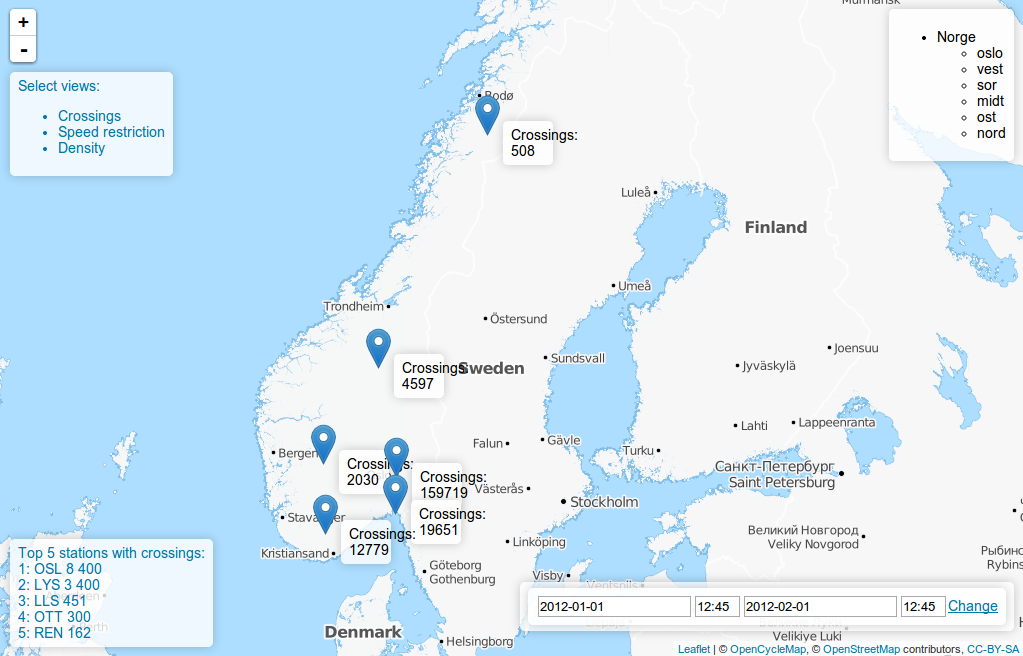
\includegraphics[width=\textwidth,center]{map_prototype.png}
	\caption[Map implementation]{Map implementation}
	\label{fig:map_prototype}
\end{figure}

\begin{figure}[h!tbp]
	\centering
	\begin{subfigure}{0.4\textwidth}
		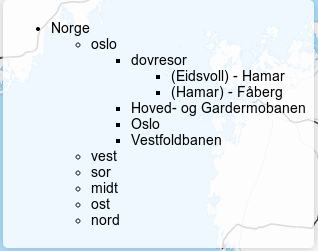
\includegraphics[width=\textwidth]{stakeholder_selection_list.png}
		\caption[Stakeholder selection list]{Stakeholder selection list}
		\label{fig:stakeholder_selection_list}
	\end{subfigure}
	\begin{subfigure}{0.3\textwidth}
		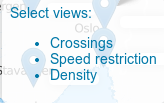
\includegraphics[width=\textwidth]{information_type_selection.png}
		\caption[Information type selection]{Information type selection}
		\label{fig:implementation_type_selection}
	\end{subfigure}
	\caption[Stakeholder selection and Information type]{Stakeholder selection and Information type}
	\label{fig:stakeholder_selection_and_information_type}
\end{figure}

\begin{figure}[h!tbp]
	\centering
	\begin{subfigure}{0.4\textwidth}
		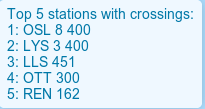
\includegraphics[width=\textwidth]{top5.png}
		\caption[Top 5 list]{Top 5 list}
		\label{fig:top_5_list}
	\end{subfigure}
	\begin{subfigure}{0.6\textwidth}
		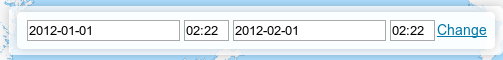
\includegraphics[width=\textwidth]{time_selection_implemented.png}
		\caption[Time selection implementation]{Time selection implementation}
		\label{fig:time_selection_implemented}
	\end{subfigure}
	\caption[Top 5 list and Time selection]{Top 5 list and Time selection}
	\label{fig:Top5_list_and_time_selection}
\end{figure}

\begin{figure}[h!tbp]
	\centering
	\begin{subfigure}{0.6\textwidth}
		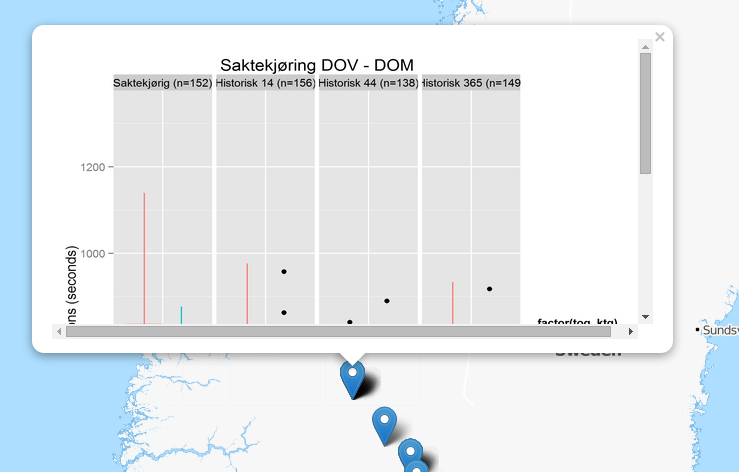
\includegraphics[width=\textwidth]{speed_restriction_presentation.png}
		\caption[Speed restriction presentation]{Speed restriction presentation}
		\label{fig:speed_restriction_presentation}
	\end{subfigure}
	\begin{subfigure}{0.25\textwidth}
		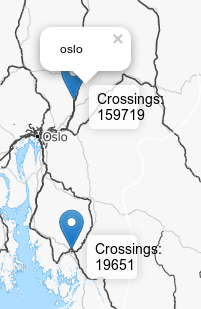
\includegraphics[width=\textwidth]{crossings_presentation.png}
		\caption[Crossings presentation]{Crossings presentation}
		\label{fig:crossings_presentation}
	\end{subfigure}
	\caption[Speed restriction and Crossings implementation]{Speed restriction and Crossings implementation}
	\label{fig:crossings_and_speed_restriction_implementation}
\end{figure}

% section prototype_functionality (end)


%\section{Prototype} % (fold)
%\label{sec:prototype}
%In this section we will describe how the developed prototype implemented the
%problem of the research question.
%
%\begin{itemize}
%	\item What are important characteristics for a stakeholder aware method to 
%	aggregate over a rich set of data?
%\end{itemize}
%
%When a important part of the system is to be aware of stakeholders and their
%requirements and needs, we found it important to have a easy way of selecting 
%different stakeholders. By having this selection,  We presented this in \Ref{sub:front_end_aggregation}.

% section prototype (end)
